\section{PD controller (Task 3)}
\label{sec:pd}

A PD controller has been designed so it satisfies the requirements shown in
\autoref{table:pd-requirements} for the cubic polynomial trajectory
\cite{TrajGener} described by \autoref{eqn:cubic-trajectory}. The controller
model is shown in \autoref{fig:PD}, the tuning of the control parameters is
described in \autoref{subsec:pd-tuning} and its behaviour in
\autoref{subsec:pd-behaviour}

\begin{equation}
    \text{Cubic polynomial trajectory } q(t) = 
    \begin{cases}
        1.5 t^2 - t^3 & t \leq 1 \\
        0.5 & \text{otherwise}
    \end{cases}
    \label{eqn:cubic-trajectory}
\end{equation}

\begin{table}
    \centering
    \begin{tabular}{c | c}
        Requirement & Value \\ \hline
        Maximal control error & $[0.01, 0.005]$
    \end{tabular}
    \\ [1ex]
    \caption{PD controller requirements}
    \label{table:pd-requirements}
\end{table}

\begin{figure}
    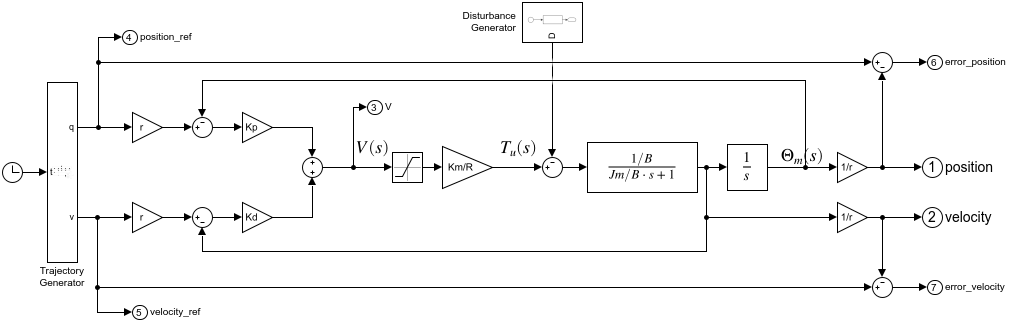
\includegraphics[width=\textwidth]{PD.slx.png}
    \caption{PD controller Simulink model}
    \label{fig:PD}
\end{figure}

\subsection{Tuning}
\label{subsec:pd-tuning}
In robotics the required dynamics should usually be possibly fast, but without
overshoots, this implies critical damping, i.e. $\zeta = 1$ \cite{SingleLink}.
That leaves the speed of response of the control system $\omega$ as the only
variable. Which is tuned in order to meet the requirements of
\autoref{table:pd-requirements}.

In order to do so, the model has been simulated with several values of $\omega$
and the maximum control error has been recorded. This maximum control error
corresponds to the maximum velocity reference, which in case of the cubic
trajectory corresponds to $t = t_f/2$ being $t$ the time and $t_f$ the end time
of the trajectory. This is exactly the middle of the movement.

\autoref{table:pd-tuning} shows the different values of the maximal control
error when modifying $\omega$. The value of $\omega = 45$ is therefore chosen to
be used for the rest of the section as it is the lowest value that satisfies
the requirements. The control system gains are calculated as described in
\citetitle{SingleLink} \cite{SingleLink} and summarized in \autoref{table:pd-constants}.

\begin{table}
    \centering
    \begin{tabular}{c | c}
        $\omega$ & Maximal control error \\ \hline\hline
        $50$ & $0.007357$ \\ \hline
        $45$ & $0.009069$ \\ \hline
        $40$ & $0.011474$ \\ \hline
    \end{tabular}
    \\ [1ex]
    \caption{PD controller tuning}
    \label{table:pd-tuning}
\end{table}

\begin{table}
    \centering
    \begin{tabular}{c | c}
        Variable & Value \\ \hline\hline
        $\omega$ & $45$ \\ \hline
        $K_p$ & $8.940857$ \\ \hline
        $K_d$ & $0.259476$ \\ \hline
    \end{tabular}
    \\ [1ex]
    \caption{PD controller parameters}
    \label{table:pd-constants}
\end{table}

\subsection{Behaviour}
\label{subsec:pd-behaviour}
The behaviour of the PD control system has been checked for the step change of
constant reference trajectory from $0$ to $0.5\text{ rad}$ as shown in
\autoref{fig:PD_step}. We obtain the expected critically damped response.

\begin{figure}
    \centering
    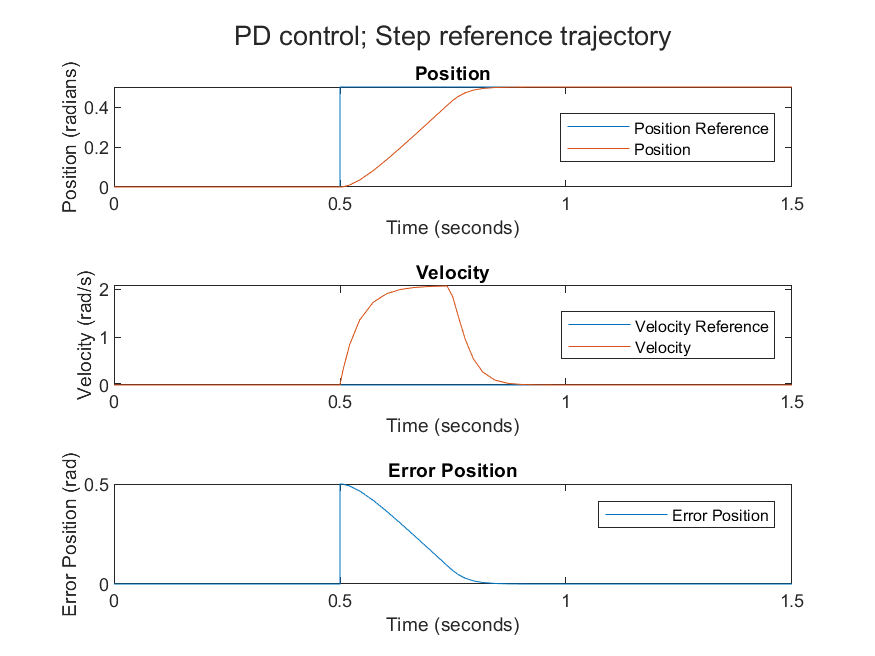
\includegraphics[width=.7\textwidth]{PD_step.png}
    \caption{Behaviour of the PD control system for the step change of constant reference trajectory from $0$ to $0.5\text{ rad}$}
    \label{fig:PD_step}
\end{figure}

\subsubsection{Undisturbed (Task 4)}
\label{subsubsec:pd-undisturbed}
The response of the PD control system has been also tested for the cubic
reference trajectory described by \autoref{eqn:cubic-trajectory} and the LSPB
\cite{TrajGener} reference trajectory described by
\autoref{eqn:LSPB-trajectory}. The results are shown in \autoref{fig:PD_cubic}
and \autoref{fig:PD_LSPB}, respectively.

Both trajectories show the expected curves for both, position and velocity. The
position error is directly related to the velocity reference and the
requirements specified in \autoref{table:pd-requirements}. It is worth to
mention that the position error for the LSPB trajectory is significantly
smaller (almost halve) than the one for the cubic polynomial trajectory. Being
both trajectory position curves quite similar this is an advantage for the LSPB
trajectory.

\begin{equation}
    \text{LSPB trajectory } q(t) = 
    \begin{cases}
        1.5625 t^2 & t \leq 0.2 \\
        0.0625 + 0.625 (t-0.2) & 0.2 \geq t \leq 0.8 \\
        0.5 - 1.5625 (t-0.6)^2 & 0.1 \geq t \leq 1 \\
        0.5 & \text{otherwise}
    \end{cases}
    \label{eqn:LSPB-trajectory}
\end{equation}

\begin{figure}
    \centering
    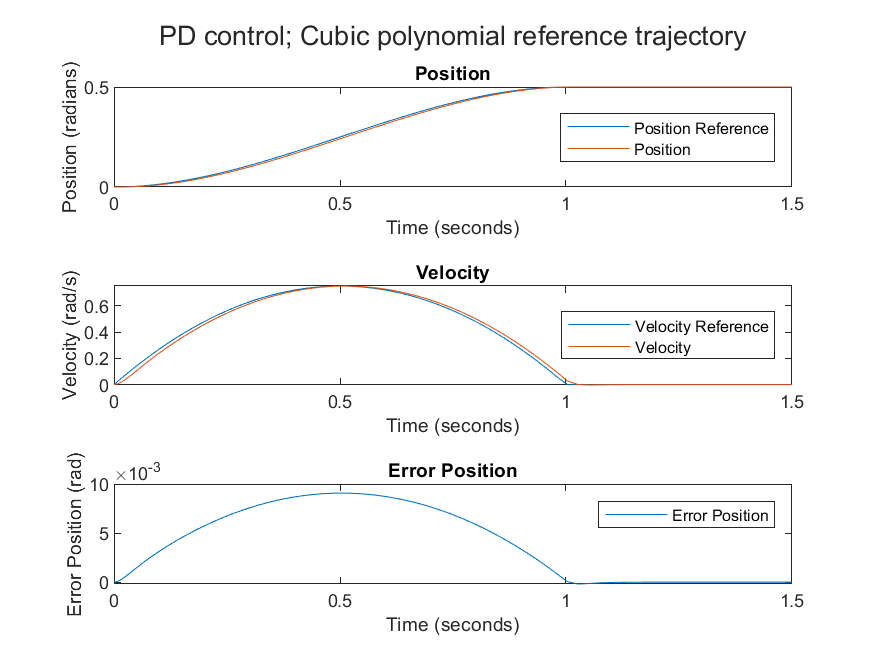
\includegraphics[width=.7\textwidth]{PD_cubic.png}
    \caption{PD control system response for the cubic polynomial trajectory}
    \label{fig:PD_cubic}
\end{figure}

\begin{figure}
    \centering
    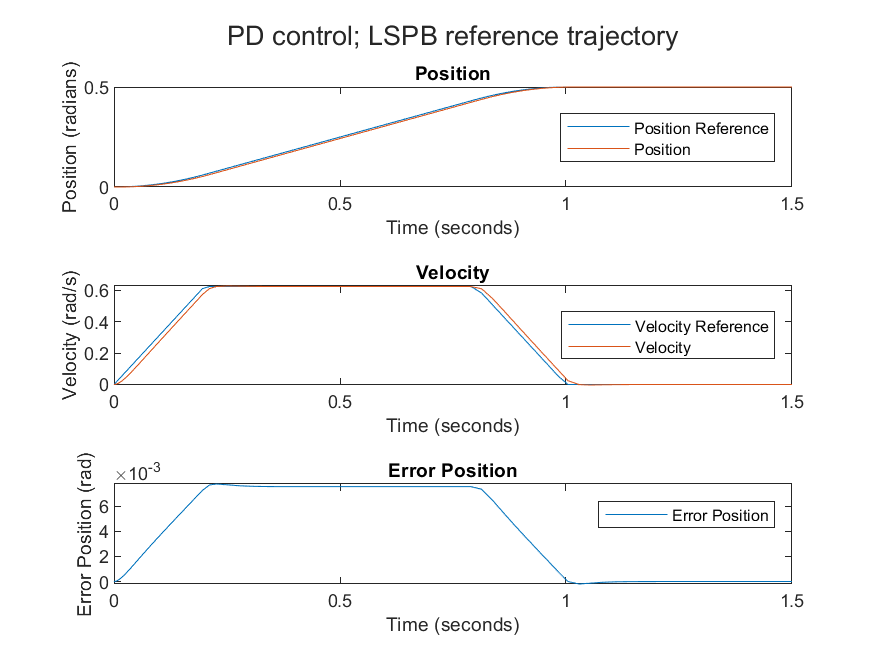
\includegraphics[width=.7\textwidth]{PD_LSPB.png}
    \caption{PD control system response for the LSPB trajectory}
    \label{fig:PD_LSPB}
\end{figure}

\subsubsection{Disturbed (Task 5)}
\label{subsubsec:pd-disturbed}
% \begin{minipage}{0.25\textwidth}
Finally, the response of the PD control system has been tested again in a
disturbed scenario with the two reference trajectories already mentioned. The
load disturbance tested is equal to $\tau_l/r = 2 N\cdot m$.
\autoref{fig:PD_cubic_disturbed} shows the results for the cubic polynomial
trajectory and \autoref{fig:PD_LSPB_disturbed} shows the results for the LSPB
trajectory.

Unlike in the undisturbed scenario, both simulations present a steady state
error in position. Being this error equal for both trajectories with a value of
$0.01379\text{ rad}$. Which matches with the equation for the steady state of a
PD control system derived in \citetitle{SingleLink} \cite{SingleLink}.
% \end{minipage}
% \begin{minipage}{0.7\textwidth}
\begin{figure}[h]
    \centering
    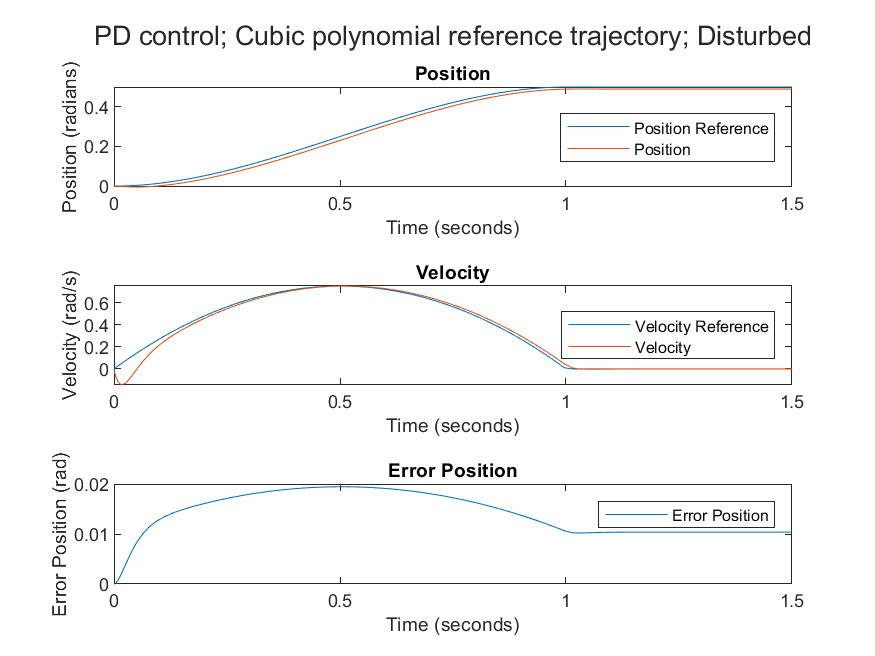
\includegraphics[width=.7\textwidth]{PD_cubic_disturbed.png}
    \caption{PD control system response for the cubic polynomial trajectory
    with disturbance}
    \label{fig:PD_cubic_disturbed}
\end{figure}
% \end{minipage}

\begin{figure}[h]
    \centering
    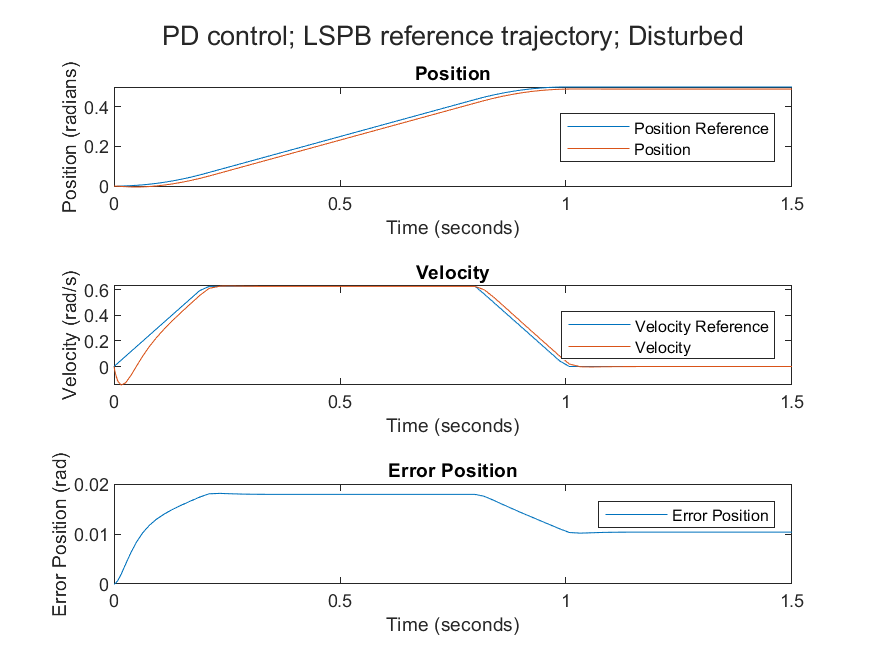
\includegraphics[width=.7\textwidth]{PD_LSPB_disturbed.png}
    \caption{PD control system response for the LSPB trajectory with disturbance}
    \label{fig:PD_LSPB_disturbed}
\end{figure}